%%%%%%%%%%%%%%%%%%%%%%%%%%%%%%%%%%%%%%%%%%%%%%%%%%%%%%%%%%%%%%%%%
%%%%%%%%%%%             GENE tutorial slides      %%%%%%%%%%%%%%%
%%%%%%%%%%% compile with: pdflatex tutorial.tex   %%%%%%%%%%%%%%%
%%%%%%%%%%%%%%%%%%%%%%%%%%%%%%%%%%%%%%%%%%%%%%%%%%%%%%%%%%%%%%%%%
\documentclass[10pt]{beamer}

\mode<presentation>
{
%  \usetheme[footnote=authortitle]{Madrid} %try Madrid, Berlin
  \usetheme{Boadilla}
%available themes: AnnArbor,Antibes, Bergen,
%Berkeley,Berlin,Boadilla,CambridgeUS,Copenhagen,Darmstadt
%Dresden,Frankfurt,Freiburg,Goettingen,Hannover,Ilmenau
%JuanLesPins,Luebeck,Madrid,Malmoe,Marburg,Montpellier
%PaloAlto,Pittsburgh,Rochester,Singapore,Szeged,Warsaw 

  %\usecolortheme{seahorse} try seahorse, whale, dolphin
  \setbeamercovered{transparent}
  \setbeamertemplate{navigation symbols}{} %Navigationsleiste ausschalten       
  %\useoutertheme[footnote=authortitle]{miniframes}
  \setbeamerfont{block title}{size=\small}
  \setbeamerfont{block content}{size=\tiny}
}

\usepackage[english]{babel}
\usepackage[T1]{fontenc} %document uses the European EC (or ec) fonts, which contain accented letters 
\usepackage{amsxtra}
\usepackage{amssymb}
\usepackage{times}
\usepackage{hyperref}
\usefonttheme[onlymath]{serif}

%new color definitions
\definecolor{myViolet}{rgb}{.7,0,.9}
\definecolor{myGreen}{rgb}{0,.4,0}
\definecolor{myGreen2}{rgb}{0,.7,0}
\definecolor{myBlue}{rgb}{0.363,0.648,1.0}
\colorlet{lila}{red!50!blue}
%new commands
\newcommand{\cB}[1]{\textcolor{blue}{#1}}
\newcommand{\cR}[1]{\textcolor{red}{#1}}
\newcommand{\cG}[1]{\textcolor{myGreen}{#1}}
\newcommand{\cV}[1]{\textcolor{orange}{#1}}
\newcommand{\cC}[1]{\textcolor{myGreen2}{#1}}
\newcommand{\cM}[1]{\textcolor{magenta}{#1}}
\usepackage{macros}

%%%%%%%%%% PDF document and titlepage info  %%%%%%%%%%%%%%%%%%%%%%%%%%%%%%%%%%%%%%%%%%%%%
\title{An introduction to \gene} 
%\subtitle{}
\author{{\it Gene Development Team}}
\institute{\href{mailto:gene@ipp.mpg.de}{gene@ipp.mpg.de}}
%\subtitle{}
%\institute[IPP]{Max-Planck-Institut f\"ur Plasmaphysik}
%\logo{
\includegraphics[width=0.05\textwidth]{gene_logo2.png}}
%\titlegraphic{
\includegraphics[width=0.25\textwidth]{gene_logo2.png}}

%%%%%%date%%%%%%%%
%\date{\today}
\day=22
\month=8
\year=2013
%%%%%%%%%%%%%%%%%%%%%%%%%%%%%%%%%%%%%%%%%%%%%%%%%%%%%%%%%%%%%%%%%%%%%%%%%%%%%%%%%%%%%%%%%

\begin{document}

%%%%%%%%%%%%%%%%%titlepage%%%%%%%%%%%%%%%%%%%%%%%%%%%%%%%%%%%%%%%%%%%%%%%%%%%%%%%%%%%%%%%
\begin{frame}[plain]
  \titlepage
\end{frame}

%%%%%%%%%%%%%%%%%%%%%%%%%%%%%%%%%%%%%%%%%%%%%%%%%%%%%%%%%%%%%%%%%%%%%%%%%%%%%%%%%%%%%%%%%

\begin{frame}[plain]
\begin{alertblock}{WARNING}
This tutorial aims at providing the basics for installing and running {\sc Gene}.
Please check
\begin{itemize}
 \item the website \url{http://gene.rzg.mpg.de}
 \item the documentation
\end{itemize}
for more recent or more detailed information regarding required libraries, input parameters, file formats etc.!
\end{alertblock}

\end{frame}


%%%%%%%%%%%%%%%%%%%%%%%%%%%%%%%%%%%%%%%%%%%%%%%%%%%%%%%%%%%%%%%%%%%%%%%%%%%%%%%%%%%%%%%%%

\begin{frame}[plain]
  \frametitle{Outline}

  \tableofcontents

\end{frame}

%%%%%%%%%%%%%%%%%%%%%%%%%%%%%%%%%%%%%%%%%%%%%%%%%%%%%%%%%%%%%%%%%%%%%%%%%%%%%%%%%%%%%%%%%

\section{What is GENE?}

\begin{frame}
  \frametitle{What is \gene?}

\begin{block}{{\sc \bf GENE} = {\bf G}yrokinetic {\bf E}lectromagnetic {\bf N}umerical {\bf E}xperiment}
\vspace{2ex}
 \begin{itemize}
  \item designed for numerical investigations of plasma microturbulence\\[2ex]
  \item solving the $\delta f$-splitted gyrokinetic system of equations using a Eulerian approach (fixed grid)
in 5D phase space\\[2ex]
  \item initial value or eigenvalue computations\\[2ex]
  \item radially local\footnote{addressed in this tutorial} (flux tube) or global (up to full torus) simulation domain\\[2ex]
  \item various interfaces to MHD equilibrium codes and transport solvers\\[2ex]
  \item massively parallelized using (mainly) MPI and OpenMP\\[2ex]
 \end{itemize}

\end{block}


\end{frame}

%%%%%%%%%%%%%%%%%%%%%%%%%%%%%%%%%%%%%%%%%%%%%%%%%%%%%%%%%%%%%%%%%%%%%%%%%%%%%%%%%%%%%%%%%

\begin{frame}
  \frametitle{Gyrokinetic system of equations I}

\begin{block}{Gyrokinetic Vlasov equation per species $\spec$ with \cC{collisions}}
\bea
\pderiv{f_\spec}{t} + \dot{\bf X}\cdot \nabla f_\spec + \dot{v}_\| \pderiv{f_\spec}{v_\|} + \dot{\mu}\pderiv{f_\spec}{\mu} = \cC{C(f_\spec,f_{\spec^\prime})}
\label{eq:vlasov}
\eea
\end{block}
\begin{minipage}{0.475\textwidth}
\begin{block}{gyrocenter position ${\bf X}$}
\vspace{-2ex}
\bea
\dot{\bf X} & = v_\| {\bf b}_0 + \frac{B_0}{B_{0\|}^*} \mvec{v}_\perp \nn
\eea
with the combined drift velocities
\bea
{\bf v}_\perp \equiv & \frac{c}{B_0^2} \bar{\mvec{\chi }}_1\times \mvec{B}_0 + \frac{\mu}{m_\spec \Omega_\spec}\mvec{b}_0\times\nabla B_0 \nn \\
& + \frac{v_\|^2}{\Omega_\spec} (\nabla\times\mvec{b})_\perp \nn
\eea
and the generalized potential 
$\bar{\mvec{\chi}} = \bar{\phi}_1 - \frac{v_\|}{c}\bar{A}_{1\|} + \frac{\mu}{q_\spec}\bar{B}_{1\|}$
\end{block}
\end{minipage}
\hspace{0.029\textwidth}
\begin{minipage}{0.475\textwidth}
\begin{block}{parallel velocity $v_\|$}
\vspace{-2ex}
\bea
\dot{v}_\| & = \frac{\dot{\mvec{X}}}{m_\spec v_\|} \cdot \left(q_\spec\bar{\mvec{E}}_1-\mu\nabla (B_0+\bar{B}_{1\|}) \right) \nn
\eea
with the electric field $\mvec{E}_1 = -\nabla \phi_1 -\frac{\mvec{b}_0}{c}\pderiv{}{t} A_{1\|}$
\end{block}
\begin{block}{magnetic moment $\mu$}
\vspace{-2ex}
\bea
\dot{\mu} = 0 \nn
\eea
\end{block}
\vspace{2ex}
... which is $\delta f$-splitted in \gene
\end{minipage}

\end{frame}

%%%%%%%%%%%%%%%%%%%%%%%%%%%%%%%%%%%%%%%%%%%%%%%%%%%%%%%%%%%%%%%%%%%%%%%%%%%%%%%%%%%%%%%%%

\begin{frame}
  \frametitle{Gyrokinetic system of equations II}

\begin{minipage}{0.35\textwidth}
\begin{block}{Gyrokinetic field equations}
{\em Poisson equation}
\bea
\nabla_\perp^2 \phi_1 = & -4\pi \sum_\spec q_\spec n_{1\spec} \nn
\eea
{\em Amp\`ere's law}
\bea
\nabla_\perp^2 A_{1\|} = & - \frac{4\pi}{c} \sum_\spec j_{1\|\spec} \nn \\
B_{1\|} = & - 4\pi \sum_\spec \frac{p_{1\perp,\spec}}{B_0} \nn
\eea
\end{block}
\ldots\, all in all a nonlinear, 5D partial integro-differential system of equations
\end{minipage}
\hspace{0.025\textwidth}
\begin{minipage}{0.605\textwidth}
\begin{block}{Relevant moments (in local approx./Fourier space)}
\vspace{-2ex}
\bea
n_{1\spec,\mvec{k}} = & \frac{2\pi B_0}{m_\spec}\!\! \int\!\!\D v_\| \D\mu \left[J_0 h_{1\spec,\mvec{k}} 
 - q_\sigma \phi_{1,\mvec{k}}  \frac{F_{0\spec}}{T_{0\spec}}\right] \nn \\
%
j_{1\|\spec,\mvec{k}} = & q_\spec \frac{2\pi B_0}{m_\spec}\!\! \int\!\!\D v_\| \D\mu \,\, v_\| 
\left[
J_0 h_{1\spec,\mvec{k}} - q_\sigma \phi_{1,\mvec{k}}  \frac{F_{0\spec}}{T_{0\spec}}
\right] \nn \\
%
p_{1\perp\spec,\mvec{k}} \equiv & \frac{2\pi B_0}{m_\spec}\!\! \int\!\!\D v_\| \D\mu \,\, \mu B_0 I_1 h_{1\spec,\mvec{k}} \nn 
\eea
% \end{block}
% \begin{block}{}
with the nonadiabatic part of $f_1$
\vspace{-1ex}
\bea
h_{1\spec} \equiv f_{1\spec} + \left[q_\spec J_0 {\phi}_1 + \mu I_1 {B}_{1\|} \right]\frac{F_{0\spec}}{T_{0\spec}} \nn
\eea
and the Bessel functions
\vspace{-1ex}
\bea
J_0 & = J_0(k_\perp\rho) \nonumber \\
I_1 & = I_1(k_\perp\rho) = 2 J_1(k_\perp\rho)/(k_\perp\rho) \nn
\eea
\end{block}

\end{minipage}



\end{frame}

%%%%%%%%%%%%%%%%%%%%%%%%%%%%%%%%%%%%%%%%%%%%%%%%%%%%%%%%%%%%%%%%%%%%%%%%%%%%%%%%%%%%%%%%%
%%%%%%%%%%%%%%%%%%%%%%%%%%%%%%%%%%%%%%%%%%%%%%%%%%%%%%%%%%%%%%%%%%%%%%%%%%%%%%%%%%%%%%%%%

\section{How to get and install the code}

\begin{frame}[plain]

\begin{center}

\begin{exampleblock}

\begin{center}
\LARGE
How to get and install GENE
\end{center}
\end{exampleblock}

\end{center}
\end{frame}

%%%%%%%%%%%%%%%%%%%%%%%%%%%%%%%%%%%%%%%%%%%%%%%%%%%%%%%%%%%%%%%%%%%%%%%%%%%%%%%%%%%%%%%%%

\begin{frame}
  \frametitle{How to get and compile the code}

\begin{block}{}
 \begin{enumerate}
  \item visit \url{http://gene.rzg.mpg.de},\\
fill and submit the short form in ``Get GENE''\\[1ex]
  \item download the code as indicated via email\\
{\tt \tiny svn co --username <USER> https://solps-mdsplus.aug.ipp.mpg.de/repos/GENE11/tags/release-<X.Y> <genedir>}\\[1ex]
  \item change to the <genedir> directory\\[1ex]
  \item call {\tt make doc} or {\tt gmake doc} to create the documentation to be found in <genedir>/doc/gene.pdf\\[1ex]
  \item call {\tt make mach\_wrapper} and check resulting string <mach>
\begin{itemize}
 \item if <mach> is other than {\tt new\_machine} and clearly related to your machine, check the header of makefiles/<mach>/<mach>.mk for modules to be loaded (skip the next slide)
 \item otherwise, you need to set up the machine dependent part of the makefile (see next slide)
\end{itemize}
 \item finally, type {\tt make} (or {\tt make -j} for parallel compilation); the resulting binary can be found in <genedir>/bin/gene\_<mach>
 \end{enumerate}
\end{block}


\end{frame}

%%%%%%%%%%%%%%%%%%%%%%%%%%%%%%%%%%%%%%%%%%%%%%%%%%%%%%%%%%%%%%%%%%%%%%%%%%%%%%%%%%%%%%%%%


\begin{frame}
  \frametitle{Setting up the makefile for an unknown machine}

\begin{block}{}
 \begin{itemize}
  \item define a meaningful name for your machine ({\tt <mach>} in the following)
\begin{itemize}
 \item either by adding an appropriate identification in {\tt <genedir>/makefiles/machine.def} (preferred; {\em one time change only}) 
 \item or by {\em permanently} setting the environment variable {\tt MACHINE}
\end{itemize}
 \item copy and rename the makefile template from {\tt \small <genedir>/makefiles/new\_machine/new\_machine.mk} to {\tt \small <genedir>/makefiles/<mach>/<mach>.mk}
 \item open {\tt \small <genedir>/makefiles/<mach>/<mach>.mk}, search for and fill at least the following tokens (check the documentation for details)
\begin{itemize}
\item the Fortran compiler {\tt COMPILER} (e.g., intel, gnu, cray, pgi, etc.)
\item {\tt FFTLIB} (fftw, mkl or essl) and the corresponding block
\item the compiler flag for double precision (search for {\tt DOUBLE\_PREC})
\item the {\bf complex} versions of {\sc Petsc} and {\sc Slepc} via {\tt PETSC\_INCLUDE}, {\tt SLEPC\_INCLUDE}, {\tt PETSC\_ARCH}; set {\tt SLEPC = yes}
\end{itemize}
% \item note: changes to {\tt \small makefiles/<mach>/<mach.mk>} might require removal of {\tt <mach.mk>} in {\tt bin}
 \item compile, run the {\em test suite} and optionally send modifications to \href{mailto:gene@ipp.mpg.de}{gene@ipp.mpg.de}
 \end{itemize}
\end{block}
\vspace{-1ex}
\begin{alertblock}{}
{\em note}: changes to {\tt \small makefiles/<mach>/<mach.mk>} require {\tt gmake distclean}
\end{alertblock}



\end{frame}

%%%%%%%%%%%%%%%%%%%%%%%%%%%%%%%%%%%%%%%%%%%%%%%%%%%%%%%%%%%%%%%%%%%%%%%%%%%%%%%%%%%%%%%%%
%%%%%%%%%%%%%%%%%%%%%%%%%%%%%%%%%%%%%%%%%%%%%%%%%%%%%%%%%%%%%%%%%%%%%%%%%%%%%%%%%%%%%%%%%

\section{Setting up a simulation}

\begin{frame}[plain]

\begin{center}

\begin{exampleblock}

\begin{center}
\LARGE
Setting up a simulation% \\
% \vspace{1ex}
% \Large
% A short introduction to the parameters file
\end{center}
\end{exampleblock}

\end{center}
\end{frame}

%%%%%%%%%%%%%%%%%%%%%%%%%%%%%%%%%%%%%%%%%%%%%%%%%%%%%%%%%%%%%%%%%%%%%%%%%%%%%%%%%%%%%%%%%

\begin{frame}[fragile]
   \frametitle{Running \gene}

\begin{exampleblock}{Example}
This would be the way how to call \gene in a shell or batch script with 8 MPI processes
 
\verb|mpiexec -n 8 ./gene_<mach>|

where \verb|mpiexec -n | might need to be substituted by {\em mpirun, aprun, poe, ...}
\end{exampleblock}

\begin{alertblock}{The input file}
The simulation parameters are set in the {\bf \tt parameters} input file which \cR{\bf \em must be located in the same directory} \& will be \cR{\bf\em read upon simulation start}
\end{alertblock}

\begin{block}{Remarks}
\begin{itemize}
 \item a strategy to organize your simulation is to create individual {\tt prob} ($\sim$ problem) directories containing {\tt parameters}, a link to the executable, batch scripts, etc. for each
 \item the command {\tt ./newprob} in {\tt <genedir>} will automatically perform those steps
\end{itemize}
 
\end{block} 
\end{frame}

%%%%%%%%%%%%%%%%%%%%%%%%%%%%%%%%%%%%%%%%%%%%%%%%%%%%%%%%%%%%%%%%%%%%%%%%%%%%%%%%%%%%%%%%%

\begin{frame}[fragile]
   \frametitle{The {\tt parameters} input file}

\begin{exampleblock}{}
Setting up the {\tt parameters} input file is the crucial part when attempting to run a simulation.
As this file uses formatted data and Fortran namelists, it can either be modified with
\begin{itemize}
 \item[(a)] the {\em text editor} of your choice
\end{itemize}
or
\begin{itemize}
 \item[(b)] the {\em graphical launcher}\\
... which furthermore tries to automatically resolve inconsistencies and assist with job submission 
\end{itemize}
\end{exampleblock} 
\end{frame}

%%%%%%%%%%%%%%%%%%%%%%%%%%%%%%%%%%%%%%%%%%%%%%%%%%%%%%%%%%%%%%%%%%%%%%%%%%%%%%%%%%%%%%%%%


% \subsection{The parameters file}
% \subsubsection{parallelization namelist}

\begin{frame}[fragile] %fragile is needed to allow verbatim environments
  \frametitle{The {\tt parameters} file - parallelization namelist}

\begin{block} %{parallelization namelist}

\begin{block}

\begin{verbatim}
&parallelization
n_procs_s =   1  !divisor of n_spec
n_procs_v =   1  !divisor of nv0 (max: 0.5*nv0)
n_procs_w =   8  !divisor of nw0
n_procs_y =   1  !divisor of nky0 (keep low)
n_procs_z =   1  !divisor of nz0 (maximum: 0.5*nz0)
/
\end{verbatim}

\end{block}
\begin{itemize}
\item This namelist sets the number of \cR{\bf MPI} processes in each dimension. 
\item Set to $\leq 0$ if the appropriate value is unknown and should be detected by \gene (will increase the initialization time)
\end{itemize}
\end{block}

\end{frame}

%%%%%%%%%%%%%%%%%%%%%%%%%%%%%%%%%%%%%%%%%%%%%%%%%%%%%%%%%%%%%%%%%%%%%%%%%%%%%%%%%%%%%%%%%

% \subsubsection{box namelist}

\begin{frame}[fragile]
  \frametitle{The {\tt parameters} file - box namelist I}

\begin{block}{Perpendicular box sizes}

\begin{block}

\verb|&box|\\
\verb|kymin    = 0.05 ! min. binormal Fourier mode|
\verb|adapt_lx =  .t. ! adapt lx to to ky mode (in linear sim's)|
\verb|lx       = 128. ! radial box width (determines |$\Delta k_x$\verb|)|
\end{block}

\begin{itemize}
\item typical {\tt kymin} value $\lesssim 0.1$ ( ly $\gtrsim 60\,\rho_\rf$) for nonlinear sim's
\item {\tt adapt\_lx = .t.} {\bf replaces} lx by 1/(ky$\cdot$shat)
 to maximize number of poloidal connections {\tt nexc} in {\bf linear} sim's
\item {\tt lx} should be $\gtrsim 60\,\rho_\rf$ and will be adjusted to 
kymin $\cdot$ shat $\cdot$ lx $\in$\Nat ;\\
alternatively, the number of poloidal connections {\tt nexc} can be specified
\end{itemize}

\begin{block}

\verb|kx_center = 0.0 ! kx center value for linear studies|
\end{block}
\begin{itemize}
\item typically, linear investigations are considering the dominant nonlinear mode which 
is typically $k_x=0$(+connections); however, particularly in strongly shaped geometries other $k_x$ 
values might be interesting, as well.
\end{itemize}


\end{block}
\end{frame}

%%%%%%%%%%%%%%%%%%%%%%%%%%%%%%%%%%%%%%%%%%%%%%%%%%%%%%%%%%%%%%%%%%%%%%%%%%%%%%%%%%%%%%%%%

\begin{frame}[fragile]
  \frametitle{The {\tt parameters} file - box namelist II}
\begin{block}{Perpendicular grid points}

\begin{block}

\verb|nx0 =  64  !number of grid points in |$x$\verb| direction|
\verb|nky0 = 16  !number of Fourier modes in |$y$\verb| direction|
\end{block}
{\em guideline} for perpendicular grid points:
\begin{itemize}
\item linearly: 
\begin{itemize}
\item at least ${\tt nx0}\gtrsim 4$ (if {\tt adapt\_lx} is true)
\item ${\tt nky0 = 1}$ - individual simulations per {\tt ky} are recommended!
\item $k_y = ${\tt kymin} (and multiples if {\tt nky0}$>1$)
\end{itemize}
\item nonlinearly:
\begin{itemize}
\item radial resolution ${\tt lx}/{\tt nx0}\lesssim 1$;
\item number of Fourier modes in binormal ($y$) direction should be
${\tt kymin}\cdot {\tt nky0}\gtrsim 1.0$ (check for vanishing growth rate with linear sim's);\\
powers of low prime numbers are recommended (better FFT performance)
\item $k_y=0,\texttt{kymin},..,\texttt{kymin}\cdot\left(\texttt{nky0}-1\right)$
\end{itemize}
\end{itemize}
remark: number of $y$ grid points in real space ${\tt ny0}=2\,{\tt nky0}$
\end{block}


\end{frame}

%%%%%%%%%%%%%%%%%%%%%%%%%%%%%%%%%%%%%%%%%%%%%%%%%%%%%%%%%%%%%%%%%%%%%%%%%%%%%%%%%%%%%%%%%

\begin{frame}[fragile]
  \frametitle{The {\tt parameters} file - box namelist III}
\begin{block}{Velocity space grid}
\begin{block}

\verb|lv =  3.0  ! box size in |$v_\parallel$\verb| direction|
\verb|lw =  9.0  ! upper simulation box end in |$\mu$\verb| direction|
\end{block}

\begin{itemize}
\item lv should be $\geq 3.0$ (in units of $v_{T\spec}=(\textbf{\cB{2}}T_{\spec 0}/m_\spec)^{1/2}$, $\spec$ : species index)
\item the parallel velocity points span the range from $-v_{T\spec}$ to $v_{T\spec}$
\item lw should be $\geq 9.0$ (in units of $T_{\spec 0}/B_\rf$)
\end{itemize}
\begin{block}

\verb|nv0 =  32  !|$v_\parallel$\verb| grid points (usually 32, 64)|
\verb|nw0 =   8  !|$\mu$\verb| grid points (typically 8, 16) |
\end{block}
\begin{itemize}
\item equidistant grid in $v_\|$, Gauss-Laguerre knots for $\mu$ grid
\end{itemize}

\end{block}

\end{frame}

%%%%%%%%%%%%%%%%%%%%%%%%%%%%%%%%%%%%%%%%%%%%%%%%%%%%%%%%%%%%%%%%%%%%%%%%%%%%%%%%%%%%%%%%%

%\part[]{Setting up a computation}

%%%%%%%%%%%%%%%%%%%%%%%%%%%%%%%%%%%%%%%%%%%%%%%%%%%%%%%%%%%%%%%%%%%%%%%%%%%%%%%%%%%%%%%%%
\begin{frame}[fragile]
  \frametitle{The {\tt parameters} file - box namelist IV}
\begin{block}%{miscellaneous}

\begin{block}

\verb|nz0 =  16  !grid points in |$z\,\,(\parallel)$\verb| direction|
\end{block}
\begin{itemize}
\item simple circular geometries: 16 or 24 parallel grid points sufficient
\item realistic MHD-equlibria: up to 100 grid points needed
\end{itemize}
\begin{block}

\verb|n_spec = 1 !number of particle species|
\end{block}
\begin{itemize}
\item n\_spec = 1: oppositely charged species is assumed to be adiabatic!
\end{itemize}
\begin{block}

\verb|x0 = 0.5 !macroscopic radial position of box center in |$L_\rf$
\end{block}
\begin{itemize}
\item req'd only if some parameters are set by MHD or profiles interfaces;\\
often given as normalized $\rho_{\rm tor}$
\end{itemize}

\end{block}
\end{frame}

%%%%%%%%%%%%%%%%%%%%%%%%%%%%%%%%%%%%%%%%%%%%%%%%%%%%%%%%%%%%%%%%%%%%%%%%%%%%%%%%%%%%%%%%%

% \subsubsection{in\_out namelist}

\begin{frame}[fragile]
  \frametitle{The {\tt parameters} file - in\_out namelist}

\begin{block}

Usually, no changes are needed in this namelist except for the following parameters:

\begin{block}

\begin{verbatim}
&in_out
diagdir = '/ptmp/exampledir'  ! output file dir
read_checkpoint = .f.
\end{verbatim}
\end{block}
\begin{itemize}
\item output files (e.g. nrg, mom, field) are written to {\tt diagdir};\\
make sure to use a high performance I/O file system
\item to continue an old simulation set {\tt read\_checkpoint} to {\tt .t.} to read an existing {\tt checkpoint} file from {\tt chptdir} (={\tt diagdir} by default) when starting the next simulation
\end{itemize}
\end{block}
\end{frame}

%%%%%%%%%%%%%%%%%%%%%%%%%%%%%%%%%%%%%%%%%%%%%%%%%%%%%%%%%%%%%%%%%%%%%%%%%%%%%%%%%%%%%%%%%

% \subsubsection{general namelist}

\begin{frame}[fragile]
  \frametitle{The {\tt parameters} file - general namelist I}

\begin{block}%{simulation type and time step}

\begin{block}

\verb|&general|
\verb|nonlinear = .t.    !switch on/off nonlinear terms|
\verb|comp_type = 'IV'   !initial(IV) or eigenvalue(EV) comput.|
\end{block}
\begin{minipage}[t]{0.575\textwidth}
\small
 \begin{block}{{\tt comp\_type = 'IV'}}

\verb|calc_dt = .t.    !switch on/off| 
\verb|                 !dt_max calculation|
\verb|dt_max  = 0.0385 !maximum time step |\\
\verb|                 !in |$L_\rf/c_\rf$
\end{block}
\begin{itemize}
\item calc\_dt = .t.
\begin{itemize}
\item PETSc/SLEPc linked $\rightarrow$ exact determination of {\tt dt\_max}
\item not linked $\rightarrow$ approximated by CFL
\end{itemize}
\item calc\_dt = .f.
\begin{itemize}
\item use {\tt dt\_max}
\end{itemize}
\end{itemize}

\end{minipage}
\hspace{0.02\textwidth}
\begin{minipage}[t]{0.385\textwidth}
 \begin{block}{{\tt comp\_type = 'EV'} (lin. only)}
\verb|n_ev = 1 !no. of EVs|
 \end{block} 
\end{minipage}
\end{block}
\end{frame}

%%%%%%%%%%%%%%%%%%%%%%%%%%%%%%%%%%%%%%%%%%%%%%%%%%%%%%%%%%%%%%%%%%%%%%%%%%%%%%%%%%%%%%%%%

\begin{frame}[fragile]
  \frametitle{The {\tt parameters} file - general namelist II}

\begin{block}{Termination conditions}

\begin{block}

\begin{verbatim}
ntimesteps =  100000 !maximum number of time steps
timelim    =   64500 !(system) time limit in sec
simtimelim =    5000 !simulation time limit
omega_prec =    1e-3 !convergence precision 
\end{verbatim}
\end{block}
\begin{itemize}
\item simulation will stop in a controlled way, if
\begin{itemize}
\item number of time steps exceeds {\tt ntimesteps}
\item simulation runs longer than {\tt timelim} seconds; \cR{set $<$ wallclock limit!}
\item simulation time in $L_\rf/c_rf$ reaches {\tt simtimelim}
\item growth rates and real frequencies are converged up to a
precision of {\tt omega\_prec} (only for linear simulations
and $\textrm{istep\_omega} > 0$).
\end{itemize}
\end{itemize}
\end{block}

\end{frame}

%%%%%%%%%%%%%%%%%%%%%%%%%%%%%%%%%%%%%%%%%%%%%%%%%%%%%%%%%%%%%%%%%%%%%%%%%%%%%%%%%%%%%%%%%

\begin{frame}[fragile]
  \frametitle{The {\tt parameters} file - general namelist III}

\begin{block}{Physics parameters}

\verb|beta         =  0.71E-02 !|$\beta_\rf\approx 403\cdot 10^{-5} n_{e19} T_{\rf ,\mathrm{keV}}/B_{\rf ,T}^2$
\verb|coll         =  0.68E-02 !normalized collision frequency|
\verb|collision_op = 'landau'  !'landau' or 'none'|
\verb|debye2       =  0.0      !normalized |$\lambda^2_{\rm Debye}/\rho_\rf^2$
\end{block}

\begin{block}{Hyper diffusion}

\begin{block}

\verb|hyp_x =   0.0   !radial hyper diffusion (keep small)|
\verb|hyp_z =   1.0   !parallel hyper diffusion|
\verb|hyp_v =   0.2   !|$v_\parallel$\verb| hyper diffusion|
\end{block}
\begin{itemize}
\item If parallel profiles %($\rightarrow$ {\em ballooning and parallel amplitude spectra diagnostics})
show {\em zig-zag} patterns and {\tt nx0} and/or {\tt nz0} cannot be increased try to adjust {\tt hyp\_z} to the maximum linear growth rate ($\sim {\cal O}(1)$)
\item to avoid recurrence effects, we recommend to set {\tt hyp\_v} to a value $\sim 0.1-0.5$
\end{itemize}
\end{block}

\end{frame}

%%%%%%%%%%%%%%%%%%%%%%%%%%%%%%%%%%%%%%%%%%%%%%%%%%%%%%%%%%%%%%%%%%%%%%%%%%%%%%%%%%%%%%%%%

\begin{frame}[fragile]
  \frametitle{The {\tt parameters} file - geometry namelist}
  

\begin{block}{Geometry}

\begin{block}

\begin{verbatim}
&geometry
magn_geometry = 's_alpha' !'slab','circular','miller'
                          !'chease','tracer_efit','gist'
\end{verbatim}
\end{block}
\begin{block}{analytic models: {\tt s\_alpha}, {\tt circular}, {\tt miller}, {\tt slab}}

\verb|q0      =  1.4   !safety factor q|
\verb|shat    =  0.796 !magnetic shear parameter|
\verb|amhd    =  0.0   !|${\alpha_{\rm MHD}=-q^2R\,(d\beta/dr)}$\verb| (-1 for automatic)|
\verb|trpeps  =  0.18  !|$r/R$ \verb| at flux tube position r|
\verb|major_R =  1.0   !major radius with respect to |$L_\rf$
\end{block}

\begin{block}{interfaces: {\tt chease}, {\tt tracer\_efit}, {\tt gist}}
minimum requirement:
\verb|geomfile  =  'examplefile' !declaration of interface file|
\end{block}
\end{block}

\end{frame}

%%%%%%%%%%%%%%%%%%%%%%%%%%%%%%%%%%%%%%%%%%%%%%%%%%%%%%%%%%%%%%%%%%%%%%%%%%%%%%%%%%%%%%%%%

\begin{frame}[fragile]
  \frametitle{The {\tt parameters} file - species namelist({\bf s})}

\begin{block}

Add a species namelist for each species:
\begin{block}

\verb|&species|\\
\verb|name = 'ions'  !species name string|\\
\verb|omn  =   2.22  !density gradient |$\omega_n=-(L_\rf/n)\,(dn/d\rho)$
\verb|omt  =   6.92  !temperature gradient |$\omega_t=-(L_\rf/T)\,(dT/d\rho)$
\verb|mass =   1.0   !mass normalized to |$m_\rf$
\verb|charge = 1     !charge norm. to elementary charge|
\verb|temp =   1.0   !temperature normalized to |$T_\rf$
\verb|dens =   1.0   !density normalized to |$n_\rf$

\verb|/|
\end{block}
\begin{itemize}
 \item check documentation for interfaces to profile files (e.g., {\tt prof\_type}
 {\tt iterdb\_file}, etc.)
\end{itemize}

\end{block}

\end{frame}

%%%%%%%%%%%%%%%%%%%%%%%%%%%%%%%%%%%%%%%%%%%%%%%%%%%%%%%%%%%%%%%%%%%%%%%%%%%%%%%%%%%%%%%%%

\begin{frame}[fragile]
  \frametitle{The {\tt parameters} file - units namelist}

\begin{block}

{\bf Optional}(!) namelist for 
\begin{itemize}
 \item denormalisation in post-processing routines
 \item consistent and automatic calculation of physics parameters as, e.g., $\beta$
\end{itemize}

\begin{block}

\verb|&units|\\
\verb|Tref = 0.9688  !reference temperature in keV|\\
\verb|nref = 4.081   !reference density in |$10^{19}\,\textrm{m}^{-3}$
\verb|mref = 2.0     !reference mass in proton mass units|
\verb|Lref = 0.6757  !reference length in m|
\verb|Bref = 2.424   !reference magnetic field (typically taken on axis) in T|

\verb|/|
\end{block}
\begin{itemize}
 \item check documentation for automatic calculation in profile file interface cases
\end{itemize}

\end{block}

\end{frame}

%%%%%%%%%%%%%%%%%%%%%%%%%%%%%%%%%%%%%%%%%%%%%%%%%%%%%%%%%%%%%%%%%%%%%%%%%%%%%%%%%%%%%%%%%

\begin{frame}[fragile]
  \frametitle{The {\tt parameters} file - automatic computations}

\begin{block}{Recommended/helpful settings if all ref. value are filled/requested(*) in {\tt units}:}

\begin{block}

\verb|&box|\\
\verb|adapt_ly = T !adapt kymin to closest n0_global for given|
\verb|             !rhostar; useful for correct visualization|

\verb|&general|\\
\verb|beta = -1    !beta consistently from ref. values|
\verb|coll = -1    !coll consistently from ref. values|
\verb|debye2 = -1  !debye2 consistently from ref. values|
\verb|zeff = -1    !zeff from data base(*)|\\[1ex]

\verb|&geometry|\\
\verb|amhd = -1    !amhd consistently from gradients and beta|
\verb|rhostar = -1 !rhostar consistently from ref. values|
\verb|dpdx_pm = -2 !pressure gradient from equilibrium (amhd)|\\[1ex]

\verb|&external_contr|\\
\verb|ExBrate = -1111 !ext. shear flow rate from data base(*)|
\verb|pfsrate = -1111 !parallel flow shear rate from data base(*)|

\end{block}
(*) requires active data base interface (see documentation/{\tt prof\_type})
\end{block}


\end{frame}

%%%%%%%%%%%%%%%%%%%%%%%%%%%%%%%%%%%%%%%%%%%%%%%%%%%%%%%%%%%%%%%%%%%%%%%%%%%%%%%%%%%%%%%%%

\begin{frame}[fragile]
  \frametitle{The {\tt parameters} file}

\begin{block}

\begin{exampleblock}{Some remarks}

\begin{itemize}
%\item The parameters shown above represent the Cyclone Base Case 
\item Information on further parameters, e.g. concerning the initial condition, 
numerical schemes, frequency of data ouput, etc. can be found in the \gene
documentation located in the {\tt /doc/} subdirectory of your \gene installation.
\end{itemize}
\end{exampleblock}

\begin{alertblock}{Convergence}

\begin{itemize}
\item In principle, each simulation has to be carefully checked for convergence with regard
to numerical parameters that is e.g. doubling box sizes and/or grid resolution for 
testing purposes.
\end{itemize}
\end{alertblock}

\end{block}

\end{frame}

%%%%%%%%%%%%%%%%%%%%%%%%%%%%%%%%%%%%%%%%%%%%%%%%%%%%%%%%%%%%%%%%%%%%%%%%%%%%%%%%%%%%%%%%%

{
\usebackgroundtemplate{
\vbox to \paperheight{\vfil\hbox to \paperwidth{\hfil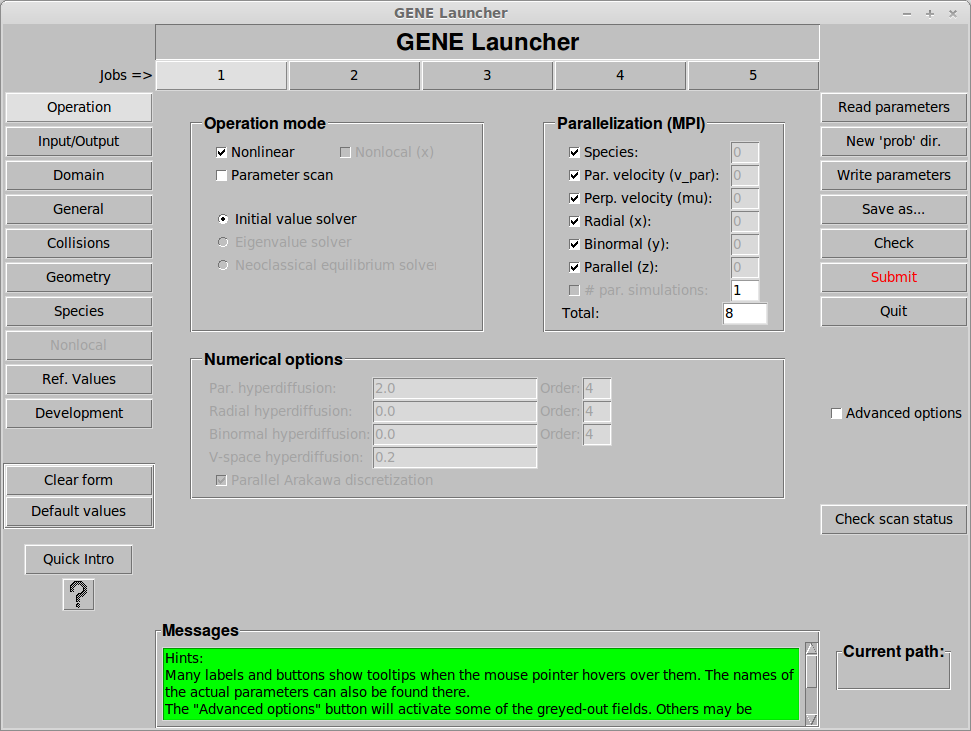
\includegraphics[width=0.8\paperwidth]{figs/launcher_operation}\hfil}\vfil}
}
\begin{frame}[fragile]
  \frametitle{Setting {\tt parameters} with the launcher I}

\vspace{5.25cm}

\begin{block}{}
\begin{itemize}
\item start python based GUI by calling \verb|./GENE-GUI.py | in {\tt <genedir>}
\item click on {\tt Default values} to fill with Cyclone-like parameters
\item set a least the number of total MPI processes and check all parallelization choices if not sure what to do here
\item click on {\tt New 'prob' dir.} for creating a new problem directory
\item \ldots and finally save your parameters here
\end{itemize}
\end{block}

\end{frame}
}

%%%%%%%%%%%%%%%%%%%%%%%%%%%%%%%%%%%%%%%%%%%%%%%%%%%%%%%%%%%%%%%%%%%%%%%%%%%%%%%%%%%%%%%%%

{
\usebackgroundtemplate{
\vbox to \paperheight{\vfil\hbox to \paperwidth{\hfil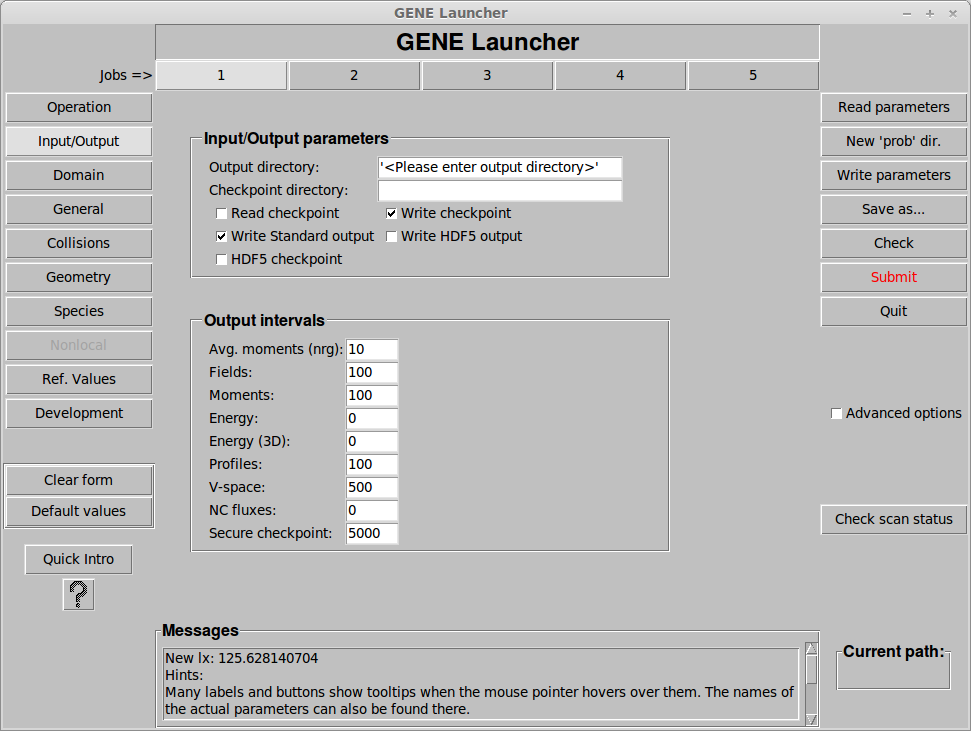
\includegraphics[width=0.8\paperwidth]{figs/launcher_inout}\hfil}\vfil}
}
\begin{frame}[fragile]
  \frametitle{Setting {\tt parameters} with the launcher II}

\vspace{7.25cm}

\begin{block}{}
\begin{itemize}
\item fill at least the Output directory
\end{itemize}
\end{block}

\end{frame}
}

%%%%%%%%%%%%%%%%%%%%%%%%%%%%%%%%%%%%%%%%%%%%%%%%%%%%%%%%%%%%%%%%%%%%%%%%%%%%%%%%%%%%%%%%%

{
\usebackgroundtemplate{
\vbox to \paperheight{\vfil\hbox to \paperwidth{\hfil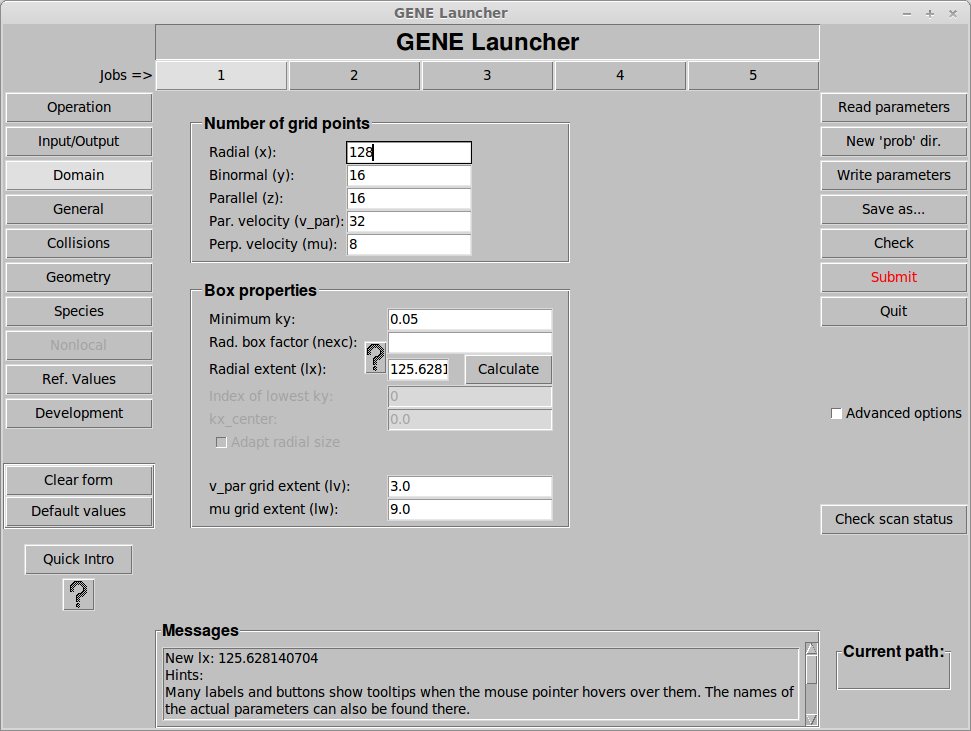
\includegraphics[width=0.8\paperwidth]{figs/launcher_domain}\hfil}\vfil}
}
\begin{frame}[fragile]
  \frametitle{Setting {\tt parameters} with the launcher III}

\vspace{5.25cm}

\begin{block}{}
\begin{itemize}
\item fill proper grid numbers (rules of thumb in previous section)
\item note that the number of poloidal connections ({\tt nexc}) can be entered directly and consistently with the radial box extension ({\tt lx})
\end{itemize}
\end{block}

\end{frame}
}

%%%%%%%%%%%%%%%%%%%%%%%%%%%%%%%%%%%%%%%%%%%%%%%%%%%%%%%%%%%%%%%%%%%%%%%%%%%%%%%%%%%%%%%%%

{
\usebackgroundtemplate{
\vbox to \paperheight{\vfil\hbox to \paperwidth{\hfil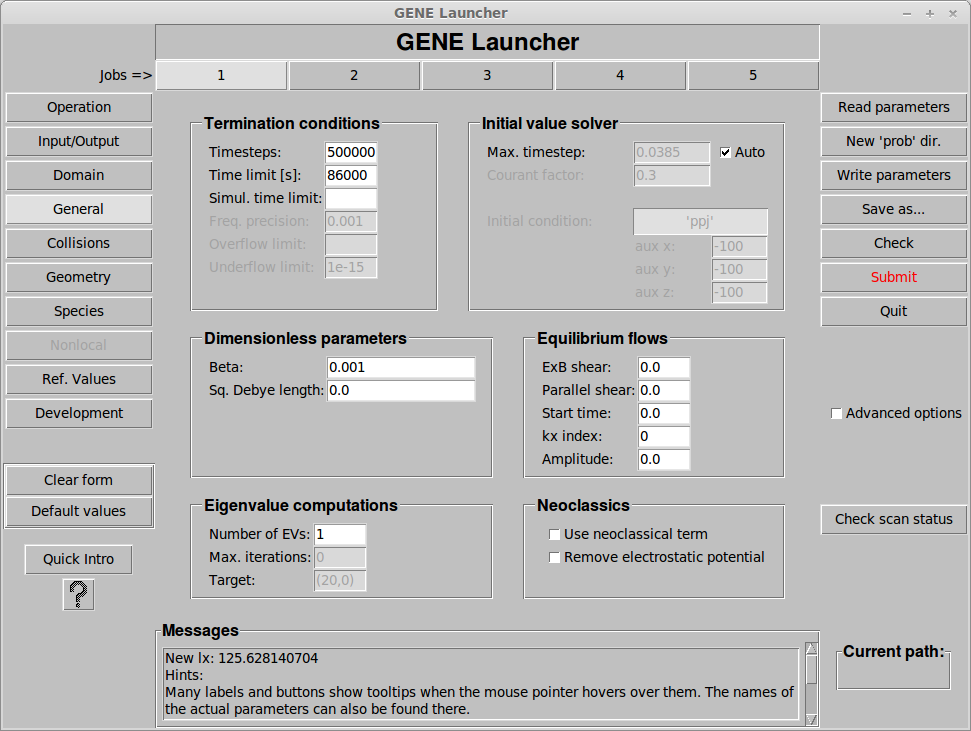
\includegraphics[width=0.8\paperwidth]{figs/launcher_general}\hfil}\vfil}
}
\begin{frame}[fragile]
  \frametitle{Setting {\tt parameters} with the launcher IV}

\vspace{5.25cm}

\begin{block}{}
\begin{itemize}
\item set time limit according to your batch system
\item fill dimensionless physical parameters as needed
\end{itemize}
\end{block}

\end{frame}
}

%%%%%%%%%%%%%%%%%%%%%%%%%%%%%%%%%%%%%%%%%%%%%%%%%%%%%%%%%%%%%%%%%%%%%%%%%%%%%%%%%%%%%%%%%

{
\usebackgroundtemplate{
\vbox to \paperheight{\vfil\hbox to \paperwidth{\hfil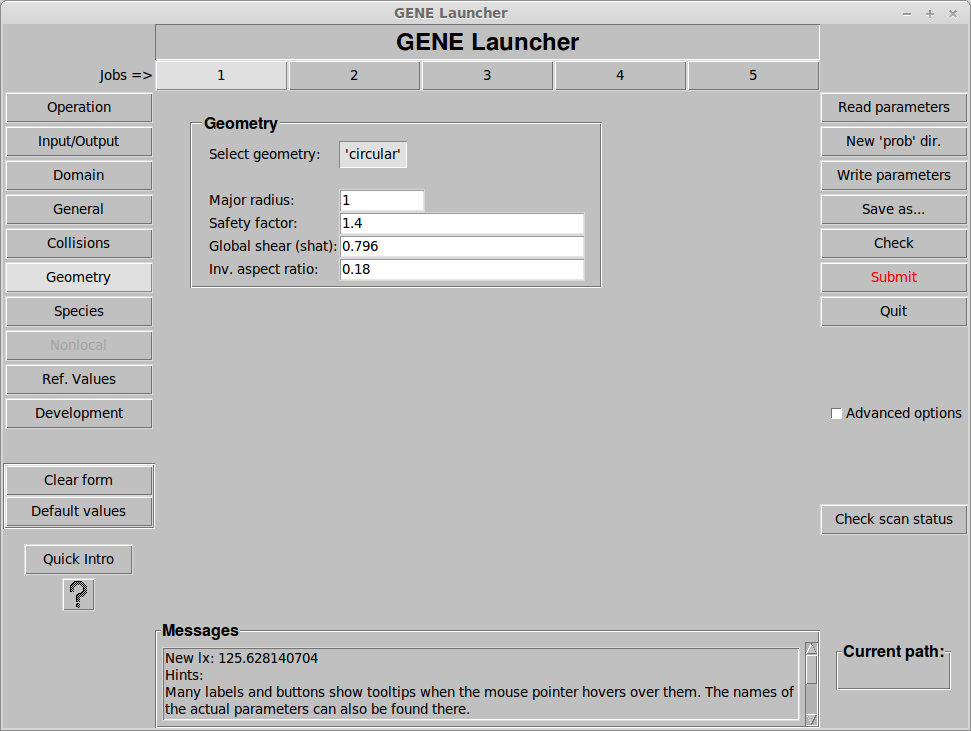
\includegraphics[width=0.8\paperwidth]{figs/launcher_geometry}\hfil}\vfil}
}
\begin{frame}[fragile]
  \frametitle{Setting {\tt parameters} with the launcher V}

\vspace{5.25cm}

\begin{block}{}
\begin{itemize}
\item choose MHD equilibrium
\item fill the requested fields
\end{itemize}
\end{block}

\end{frame}
}

%%%%%%%%%%%%%%%%%%%%%%%%%%%%%%%%%%%%%%%%%%%%%%%%%%%%%%%%%%%%%%%%%%%%%%%%%%%%%%%%%%%%%%%%%

{
\usebackgroundtemplate{
\vbox to \paperheight{\vfil\hbox to \paperwidth{\hfil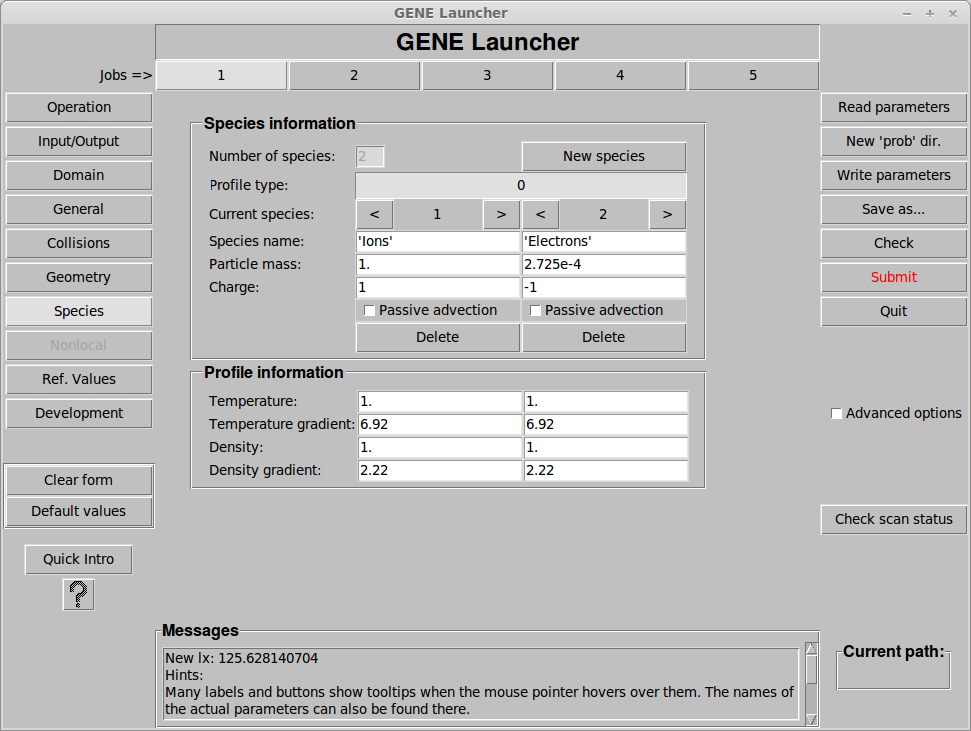
\includegraphics[width=0.8\paperwidth]{figs/launcher_species}\hfil}\vfil}
}
\begin{frame}[fragile]
  \frametitle{Setting {\tt parameters} with the launcher VI}

\vspace{5.25cm}

\begin{block}{}
\begin{itemize}
\item add and remove species using the 'New species' and 'Delete' buttons
\item fill the corresponding list for each species
\item to read numerical profiles select the appropriate profile type, and fill the requested fields
\end{itemize}
\end{block}

\end{frame}
}

%%%%%%%%%%%%%%%%%%%%%%%%%%%%%%%%%%%%%%%%%%%%%%%%%%%%%%%%%%%%%%%%%%%%%%%%%%%%%%%%%%%%%%%%%

{
\usebackgroundtemplate{
\vbox to \paperheight{\vfil\hbox to \paperwidth{\hfil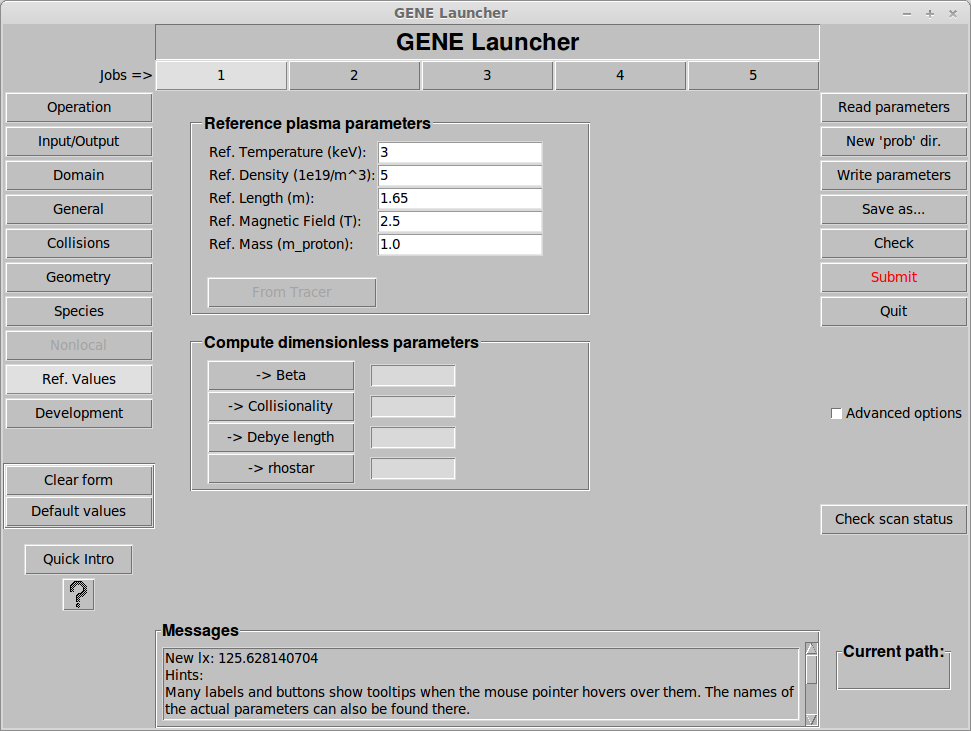
\includegraphics[width=0.8\paperwidth]{figs/launcher_reference}\hfil}\vfil}
}
\begin{frame}[fragile]
  \frametitle{Setting {\tt parameters} with the launcher VII}

\vspace{5.25cm}

\begin{block}{}
\begin{itemize}
\item optionally fill reference values for denormalization in the post-processing
\item optionally set dependent dimensionless input parameters self-consistently by clicking the buttons
\end{itemize}
\end{block}

\end{frame}
}

%%%%%%%%%%%%%%%%%%%%%%%%%%%%%%%%%%%%%%%%%%%%%%%%%%%%%%%%%%%%%%%%%%%%%%%%%%%%%%%%%%%%%%%%%

{
\usebackgroundtemplate{
\vbox to \paperheight{\vfil\hbox to \paperwidth{\hfil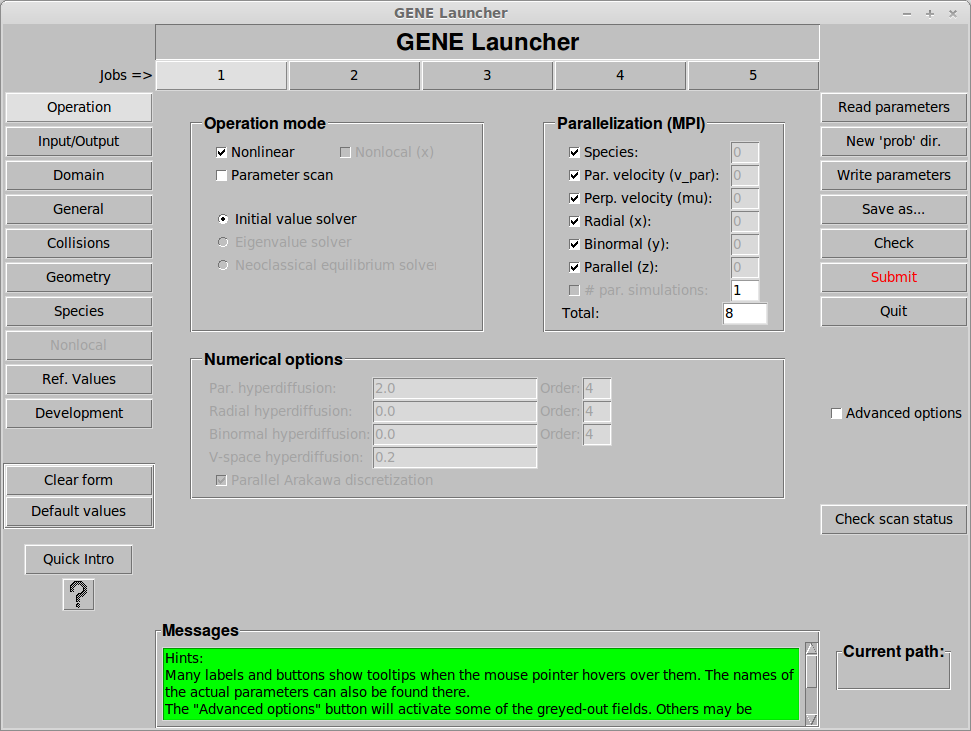
\includegraphics[width=0.8\paperwidth]{figs/launcher_operation}\hfil}\vfil}
}
\begin{frame}[fragile]
  \frametitle{Setting {\tt parameters} with the launcher VIII}

\vspace{6.25cm}

\begin{block}{}
\begin{itemize}
\item Check
\item and Submit\\
(this requires a {\tt launcher.cmd} batch script template in \verb|makefiles/<mach>/|)
\end{itemize}
\end{block}

\end{frame}
}

%%%%%%%%%%%%%%%%%%%%%%%%%%%%%%%%%%%%%%%%%%%%%%%%%%%%%%%%%%%%%%%%%%%%%%%%%%%%%%%%%%%%%%%%%

\begin{frame}[fragile]
  \frametitle{The {\tt scanscript}}

\begin{alertblock}{A well known problem ...}
The need to scan over multiple parameter values, e.g., to determine a threshold
\end{alertblock}

\begin{block}{Solution}
\begin{itemize}
 \item add Fortran comments as follows to the desired parameters, e.g., \\
  \verb| omt = 6.9 !scanlist:0.0,3.0,4.0,5.0,6.9| \\
  \ldots representing a scan over a list of temperature gradient values\\
  This also works in the launcher tool!\\[1ex]
 \item use the proper system call!
\begin{itemize}
\item either just activate {\em parameter scan} in the launcher
\item or replace \verb|mpiexec -n <NMPI> ./gene_<mach>| in your batch script by
 \verb|./scanscript -np <NMPI> -ppn <MINPROCS>|\\
 \verb|<NMPI>|: total number of mpi processes\\
 \verb|<MINPROCS>|: minimum number of processors per simulation 
 (scanscript might run several simulations in parallel for optimum efficiency)
\end{itemize}
\item check \verb|./scanscript --help| and the documentation for further options 
and output file arrangement
\end{itemize}
 
\end{block}


\end{frame}


%%%%%%%%%%%%%%%%%%%%%%%%%%%%%%%%%%%%%%%%%%%%%%%%%%%%%%%%%%%%%%%%%%%%%%%%%%%%%%%%%%%%%%%%%
%%%%%%%%%%%%%%%%%%%%%%%%%%%%%%%%%%%%%%%%%%%%%%%%%%%%%%%%%%%%%%%%%%%%%%%%%%%%%%%%%%%%%%%%%

\section{Analyzing and post-processing}

\begin{frame}[plain]

\begin{center}

\begin{exampleblock}

\begin{center}
\LARGE
Analyzing and post-processing% \\
% \vspace{1ex}
% \Large
% A short introduction to the parameters file
\end{center}
\end{exampleblock}

\end{center}
\end{frame}

%%%%%%%%%%%%%%%%%%%%%%%%%%%%%%%%%%%%%%%%%%%%%%%%%%%%%%%%%%%%%%%%%%%%%%%%%%%%%%%%%%%%%%%%%

\section{The Diagnostics Tool}

\begin{frame}
  \frametitle{The Diagnostics Tool}

\begin{figure}
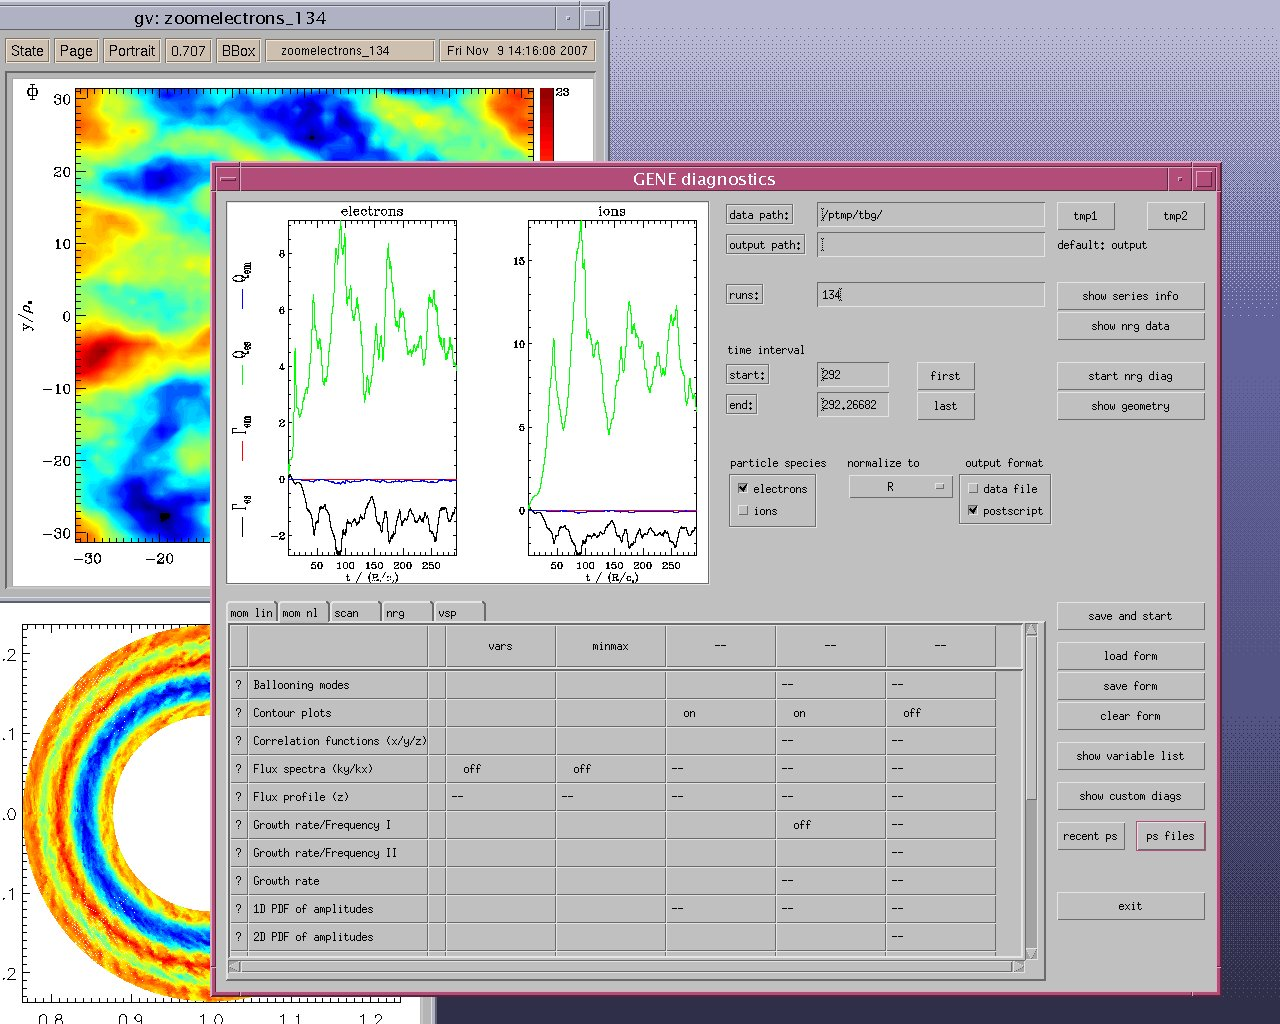
\includegraphics[height=0.6\textwidth]{figs/diag_screenshot.jpg}
\end{figure}

\end{frame}

%%%%%%%%%%%%%%%%%%%%%%%%%%%%%%%%%%%%%%%%%%%%%%%%%%%%%%%%%%%%%%%%%%%%%%%%%%%%%%%%%%%%%%%%%

\begin{frame}[fragile]
  \frametitle{The Diagnostics Tool I}

\begin{block}{Starting}

\begin{itemize}
\item regular IDL version (requires IDL licence):\\
full functionality, user can customize diagnostics
\item IDL Virtual machine version:\\
no manipulation of source possible; IDL VM is free
\item Both versions: platform-independent (Unix, Mac OS, Win32; for latter, see documentation)
\end{itemize}

\vspace{0.2cm}

\begin{itemize}
\item IDL: start \verb|idl| in diagnostics directory, then run \verb|@diag|
\item IDL VM: start \verb|idl -vm=vm_diag.sav|
\end{itemize}

\begin{alertblock}{Warning}
The diagnostics tool needs to be run on a platform from which one's data is accessible via
the file system!
\end{alertblock}

\end{block}

\end{frame}

%%%%%%%%%%%%%%%%%%%%%%%%%%%%%%%%%%%%%%%%%%%%%%%%%%%%%%%%%%%%%%%%%%%%%%%%%%%%%%%%%%%%%%%%%

{
\usebackgroundtemplate{
\vbox to \paperheight{\vfil\hbox to \paperwidth{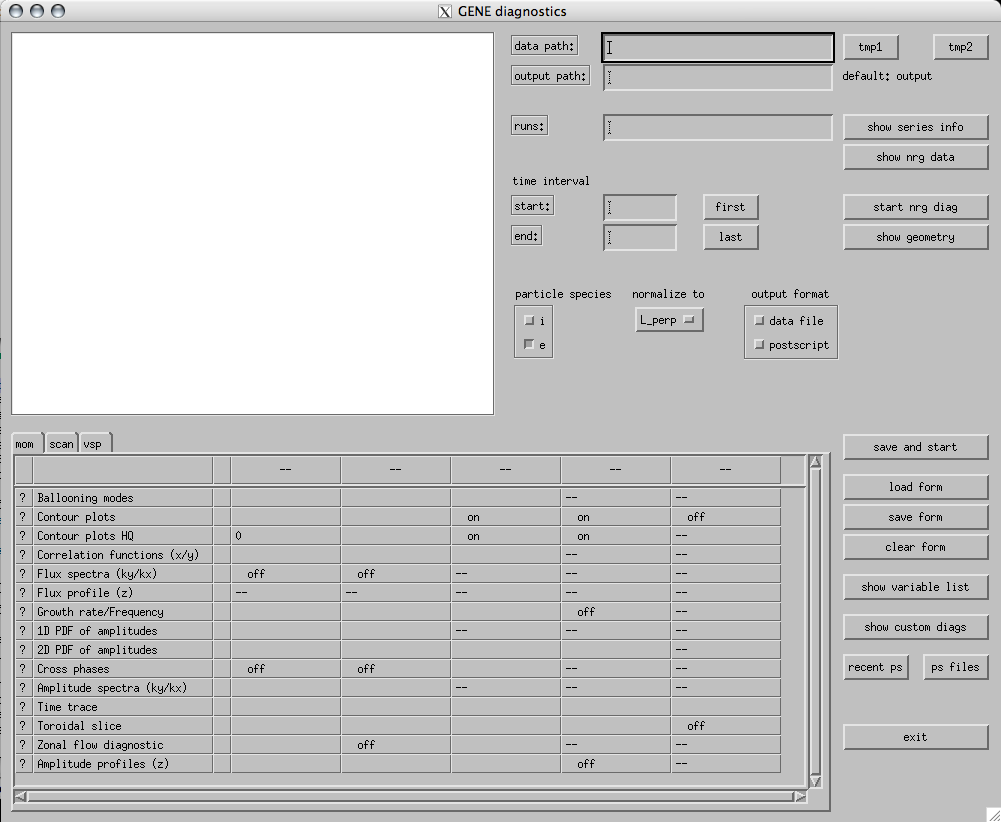
\includegraphics[width=12cm]{figs/diag_new}\hfil}\vfil}
}

%\begin{frame}{test}

%\end{frame}

\begin{frame}[fragile]
  \frametitle{{ }\\The Diagnostics Tool II\\Graphical User Interface}

\vspace{3cm}

%\begin{block}{The Graphical User Interface}
%{\bf
%\begin{minipage}{5cm}
%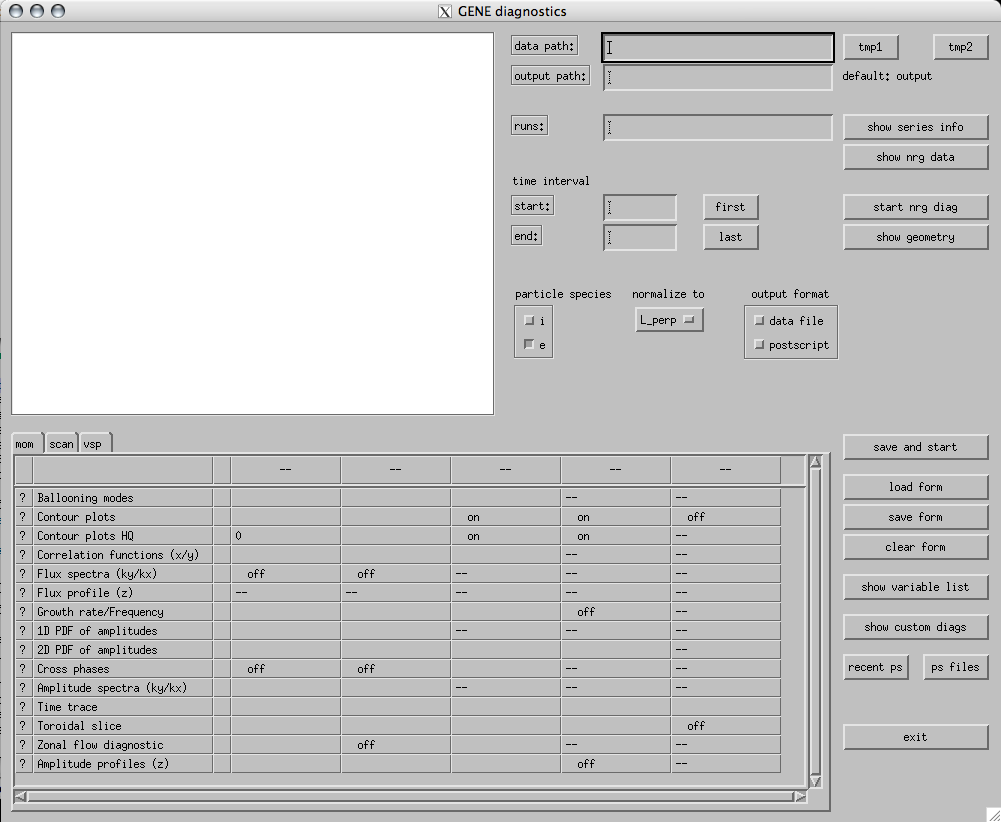
\includegraphics[width=5cm]{figs/diag_new.png}
%\end{minipage}
%\begin{minipage}{8cm}
\begin{block}{}
\begin{itemize}
%\item \verb|data path|: relative or absolute
%\item \verb|tmp| buttons: customizable paths\\
%\includegraphics[width=7cm]{figs/diag_tmp2.png}
%\item \verb|output path|: destination for ps/data/\dots
\item \verb|runs|: e.g.~\verb|256,261-264,270+|, \verb|[enter]| rec'd
\item \verb|series info|: important parameters $\rightarrow$ window
\item \verb|nrg data|: nrg time traces $\rightarrow$ window
%\item \verb|time interval|: analysis time window for nrg/mom/\dots
\item \verb|nrg diag|: growth rate and saturation analysis
\item \verb|geometry|: parallel variation $\rightarrow$ window
%\item \verb|species|: species to analyze
%\item \verb|normalize|: applies to show/nrg diag/mom/\dots
%\item \verb|output format|: for non-window analyses
\end{itemize}
\end{block}

\end{frame}

%%%%%%%%%%%%%%%%%%%%%%%%%%%%%%%%%%%%%%%%%%%%%%%%%%%%%%%%%%%%%%%%%%%%%%%%%%%%%%%%%%%%%%%%%

\begin{frame}[fragile]
  \frametitle{}%The Diagnostics Tool II -- GUI}

\vspace{-0.2cm}  

\begin{block}{}
\begin{itemize}
\item \verb|diag table|:\\
\vspace{-0.2cm}
\begin{itemize}
\item tabs: analyze mom/scan/vsp files
\item \verb|?|: help text
%\item name: title of diag
\item activation status: if active, \verb|X|
%\item parameters: \verb|on|/\verb|off| or value(s)
\end{itemize}
\vspace{-0.2cm}
\item \verb|save and start|: selected mom/scan/vsp diags
%\item \verb|load|/\verb|save|/\verb|clear|: GUI (\verb|internal/guiform|)
\item \verb|variable list|: variable $\leftrightarrow$ number for diag table par's
%\item \verb|custom diags|: recompiled on start, see documentation
\item \verb|recent ps|: ps files in \verb|gv| after \verb|save and start|
%\item \verb|ps files|: open dialog, output directory
\item \verb|ps files|: open dialog, output directory
\item \verb|exit|: close, GUI state not saved
\end{itemize}
%\end{minipage}
%}
%\end{block}
\end{block}

\vspace{4cm}

\end{frame}
}

%%%%%%%%%%%%%%%%%%%%%%%%%%%%%%%%%%%%%%%%%%%%%%%%%%%%%%%%%%%%%%%%%%%%%%%%%%%%%%%%%%%%%%%%%

\begin{frame}[fragile]
  \frametitle{The Diagnostics Tool III}

\begin{block}{Using the Diagnostics Tool}

\begin{itemize}
\item preliminaries (to check run parameters and/or time evolution): run number,
\verb|[enter]|, \verb|normalization|, \verb|show series info|/\verb|show nrg data|
\item full \verb|nrg| analysis: time window, \verb|species|, \verb|normalization|,
\verb|output format|, \verb|start nrg diag|, (hourglass cursor), \verb|recent ps|
\item full \verb|mom|/\verb|scan|/\verb|vsp| analysis: time window, \verb|species|,
\verb|normalization|, \verb|output format|, select diags in table
(check third column with \verb|X|), fill in diag parameters, repeat this with other diags,
\verb|save and start|, wait for completion dialog, \verb|recent ps|
\end{itemize}

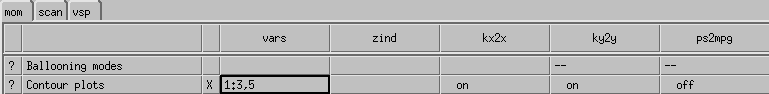
\includegraphics[width=14cm]{figs/diag_table_cont.png}

\end{block}

\end{frame}

%%%%%%%%%%%%%%%%%%%%%%%%%%%%%%%%%%%%%%%%%%%%%%%%%%%%%%%%%%%%%%%%%%%%%%%%%%%%%%%%%%%%%%%%%

\begin{frame}[fragile]
  \frametitle{The Diagnostics Tool III}

\begin{block}{Using the Diagnostics Tool}

\begin{itemize}
\item for help with specific diags, press \verb|?| next to diag name $\rightarrow$
general description, parameters info
\item custom diags: can modify with Diagnostics Tool open, auto-recompiled on
\verb|save and start| (only with full IDL)
\end{itemize}

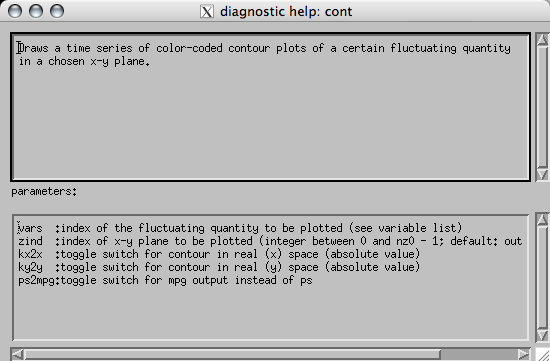
\includegraphics[width=8cm]{figs/diag_cont_help.png}

\end{block}

\end{frame}

%%%%%%%%%%%%%%%%%%%%%%%%%%%%%%%%%%%%%%%%%%%%%%%%%%%%%%%%%%%%%%%%%%%%%%%%%%%%%%%%%%%%%%%%%

\begin{frame}[fragile]
  \frametitle{The Diagnostics Tool IV}

\begin{block}{Scans and Data Output}

Scan analysis: $\quad$ \verb|runs| -- ignored; \verb|sort method| -- \verb|0|

Data output:
\begin{itemize}
\item (plain text) data files with predefined output
\item for modification/specific info, change source: \verb|prog/[diag].pro|\\
$\rightarrow$ search for \verb|dat=|\\
$\rightarrow$ modify content (e.g., variables) to be written to file
\end{itemize}
\end{block}

\begin{block}{Reality Check: Which Diags Are Essential?}
\begin{itemize}
\item linear runs: \verb|Growth rate/Frequency|, \verb|Amplitude spectra|, \verb|Amplitude profiles|
\item nonlinear runs: \verb|Contour plots|, \verb|Flux spectra|, \verb|Flux profile|
\end{itemize}
\end{block}

Note: for eigenvalue analysis, enter \verb|-[EV number]| as time window

\end{frame}

%%%%%%%%%%%%%%%%%%%%%%%%%%%%%%%%%%%%%%%%%%%%%%%%%%%%%%%%%%%%%%%%%%%%%%%%%%%%%%%%%%%%%%%%%

\begin{frame}[plain]

\begin{center}

\begin{exampleblock}

\begin{center}
\LARGE
Some basic checks \& examples% \\
% \vspace{1ex}
% \Large
% A short introduction to the parameters file
\end{center}
\end{exampleblock}

\end{center}
\end{frame}

%%%%%%%%%%%%%%%%%%%%%%%%%%%%%%%%%%%%%%%%%%%%%%%%%%%%%%%%%%%%%%%%%%%%%%%%%%%%%%%%%%%%%%%%%

\begin{frame}
  \frametitle{Check the metric coefficients for realistic geometries}

\begin{figure}
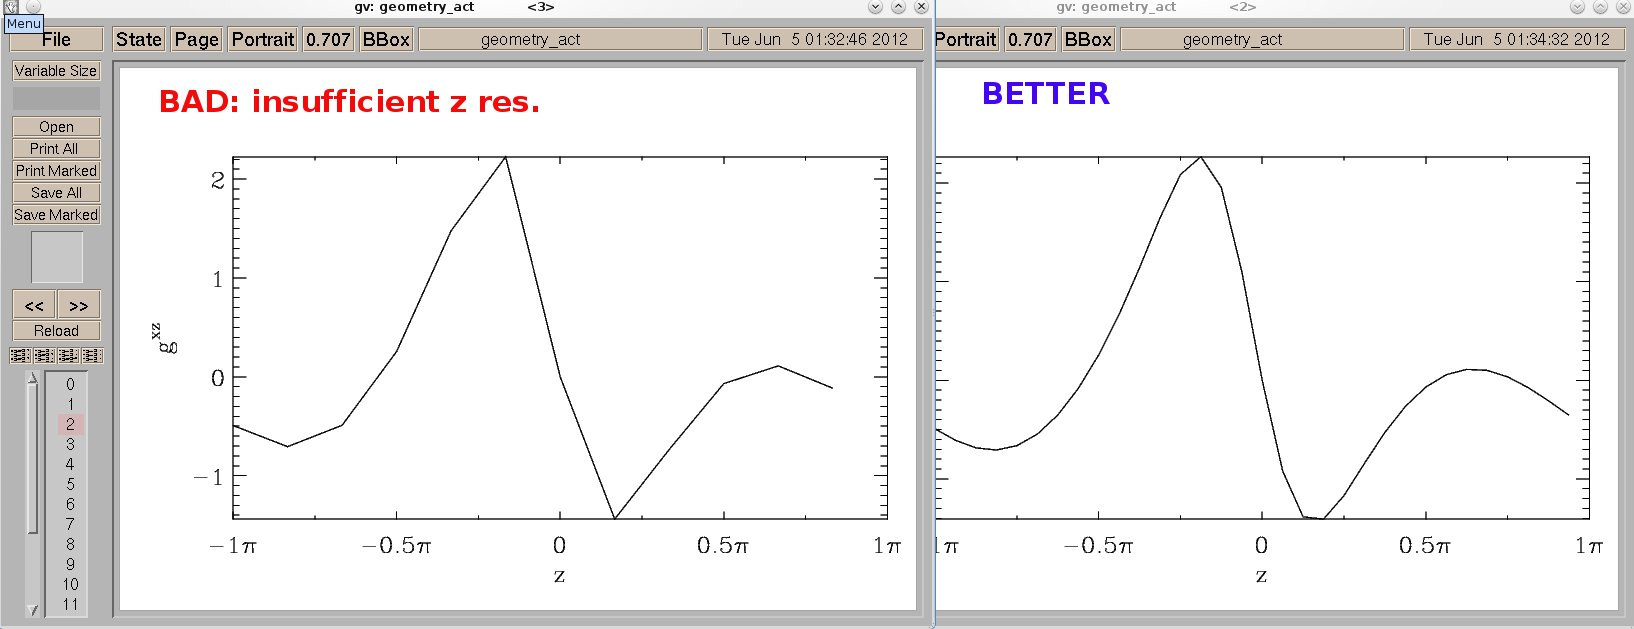
\includegraphics[width=0.9\textwidth]{figs/geometry.jpg}
\end{figure}

\begin{block}{}
\begin{itemize}
 \item click ``show geometry''
 \item check {\em smoothness}
 \item if jagged, increase {\tt nz0}
\end{itemize}

\end{block}

\end{frame}

%%%%%%%%%%%%%%%%%%%%%%%%%%%%%%%%%%%%%%%%%%%%%%%%%%%%%%%%%%%%%%%%%%%%%%%%%%%%%%%%%%%%%%%%%

\begin{frame}
  \frametitle{Linear: Check ballooning structure}

\begin{figure}
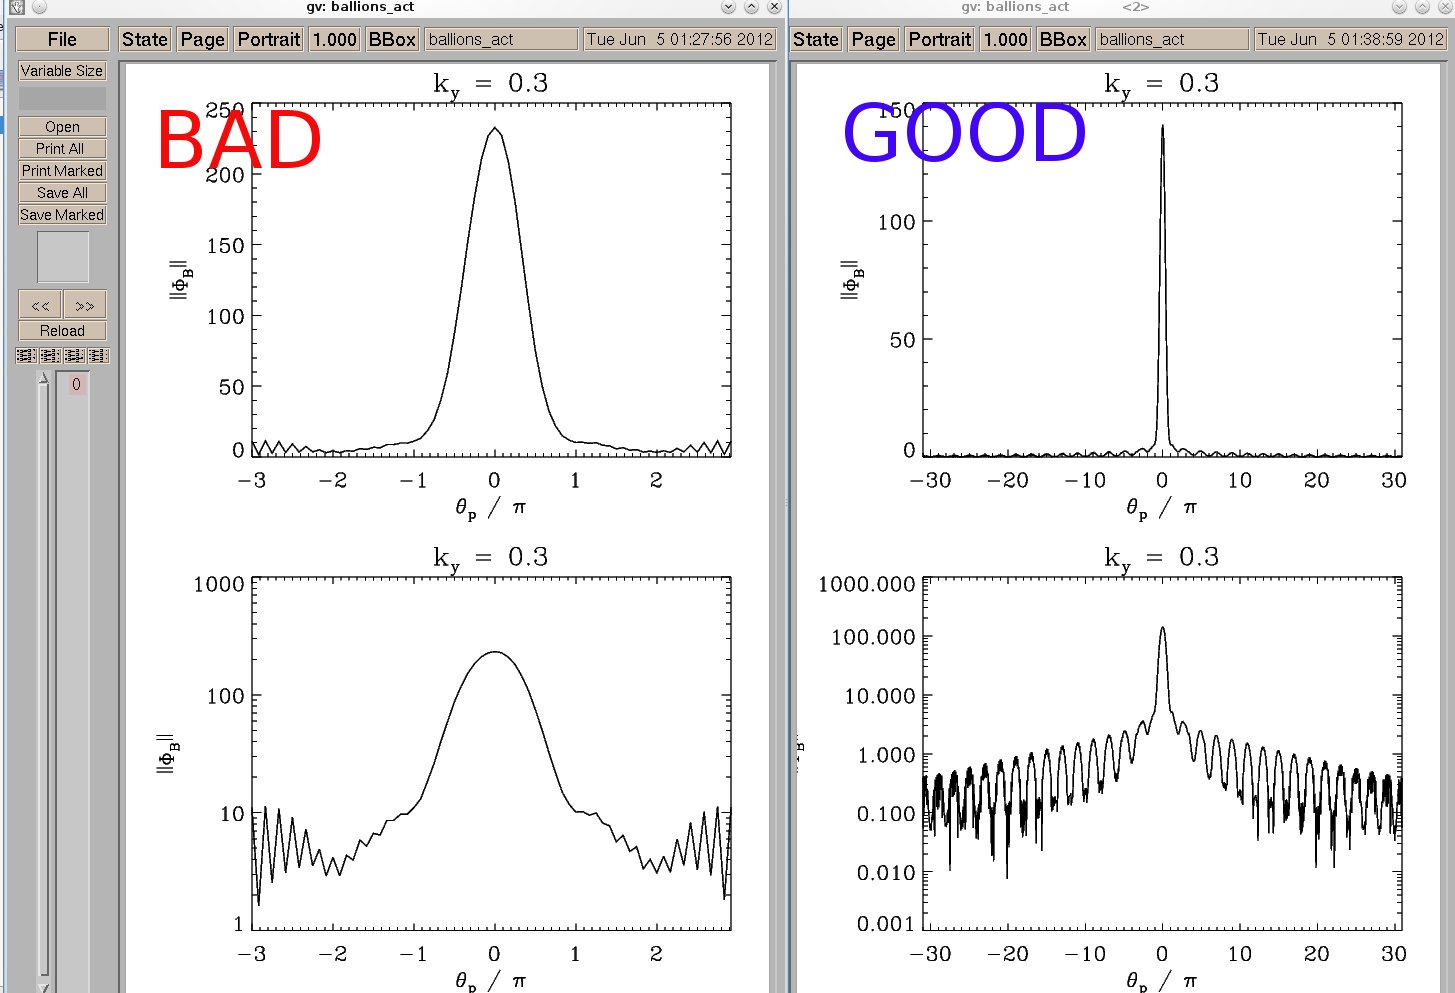
\includegraphics[height=0.6\textheight]{figs/ballooning.jpg}
\end{figure}

\begin{block}{}
\begin{itemize}
 \item select ``Ballooning modes'' for the last time steps
 \item mode structure should significantly fall off; if not increase {\tt nx0}
 \item if still jagged afterwards, increase {\tt nz0} or (carefully) apply {\tt hyp\_z}
\end{itemize}

\end{block}

\end{frame}

%%%%%%%%%%%%%%%%%%%%%%%%%%%%%%%%%%%%%%%%%%%%%%%%%%%%%%%%%%%%%%%%%%%%%%%%%%%%%%%%%%%%%%%%%

\begin{frame}
  \frametitle{Nonlinear: Check flux spectra}

\begin{figure}
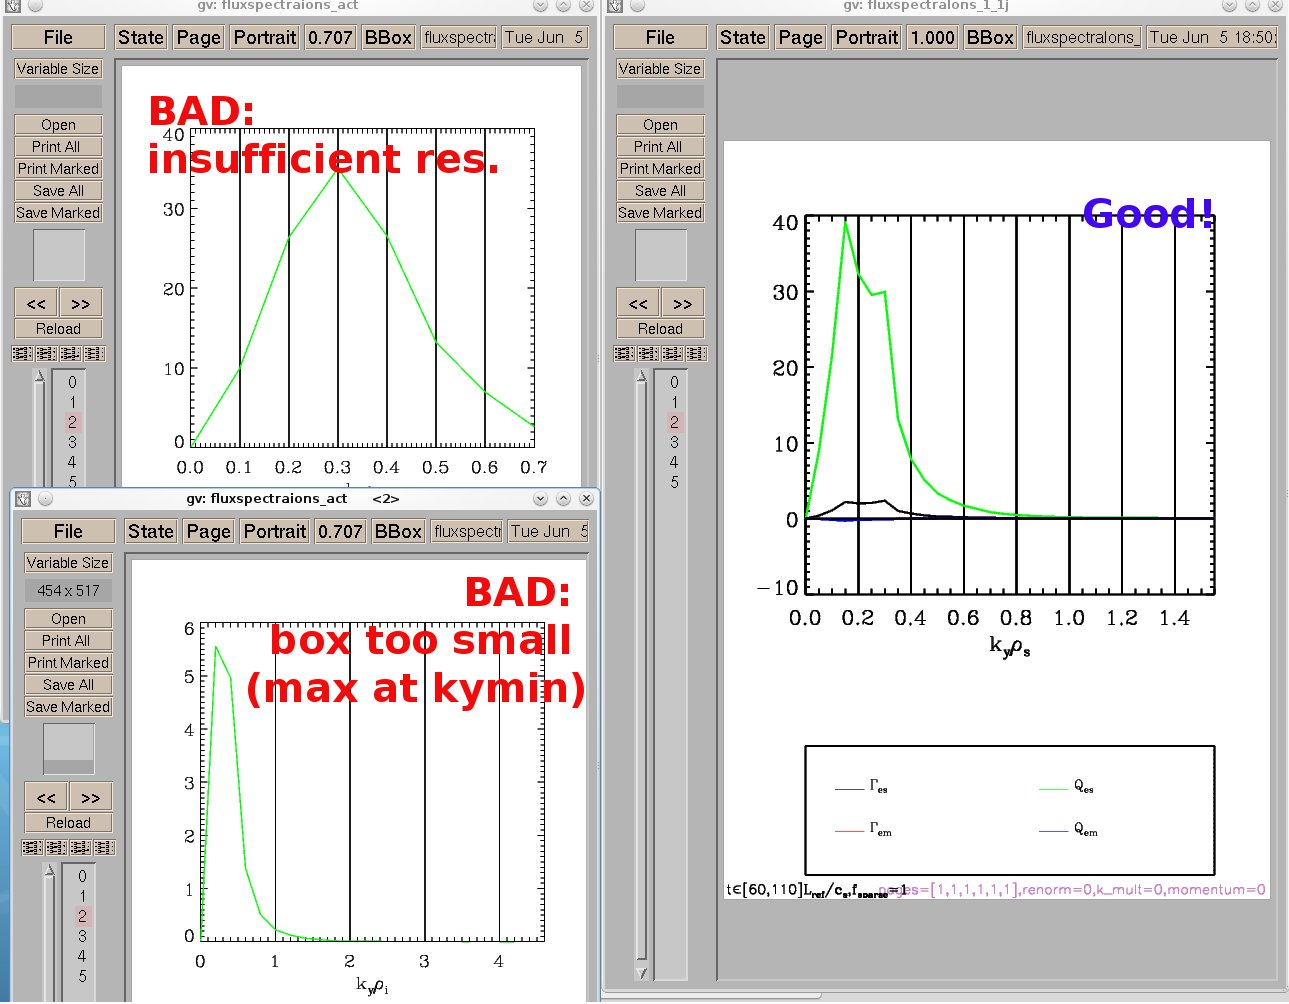
\includegraphics[height=0.6\textheight]{figs/fluxspectra.jpg}
\end{figure}

\begin{block}{}
\begin{itemize}
 \item select ``Flux Spectra (ky/kx)''
 \item (!)use long time windows {\em beyond the overshoot} for nonlinear analysis(!)
 \item transport should be small at highest $k_y, k_x$, otherwise increase {\tt nx0}, {\tt nky0}
 \item transport should not peak at lowest $k$, increase box size {\tt lx}/decrease {\tt kymin} else
\end{itemize}

\end{block}


\end{frame}

%%%%%%%%%%%%%%%%%%%%%%%%%%%%%%%%%%%%%%%%%%%%%%%%%%%%%%%%%%%%%%%%%%%%%%%%%%%%%%%%%%%%%%%%%

\begin{frame}
  \frametitle{Nonlinear: Check amplitude spectra}

\begin{figure}
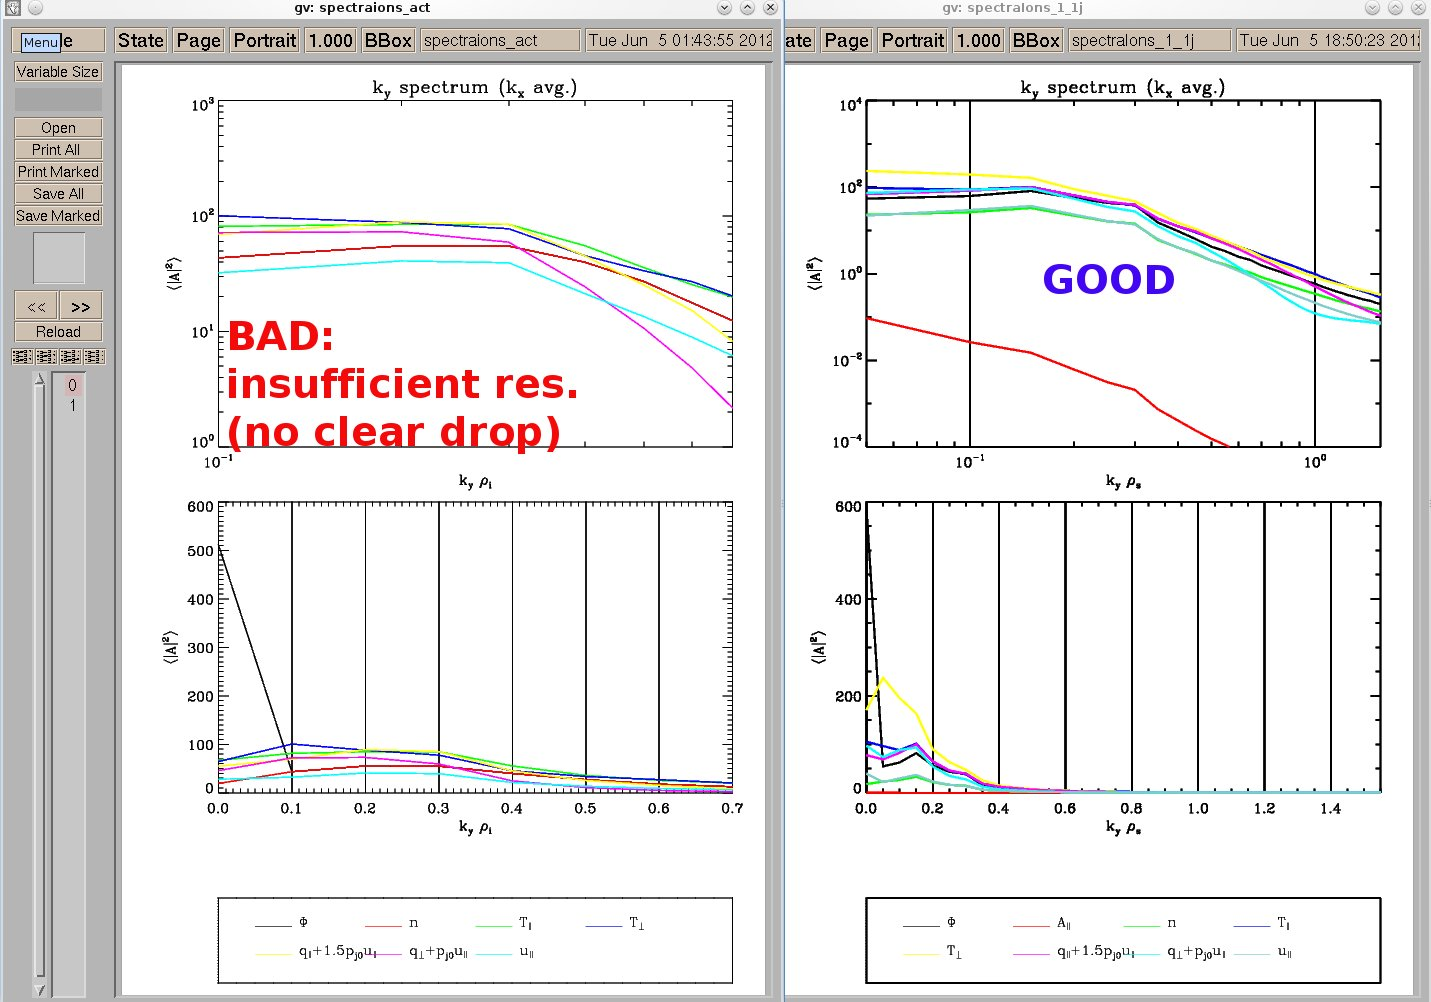
\includegraphics[height=0.6\textheight]{figs/spectra.jpg}
\end{figure}

\begin{block}{}
\begin{itemize}
 \item select ``Amplitude spectra (ky/kx)''
 \item (!)use long time windows {\em beyond the overshoot} for nonlinear analysis(!)
 \item observables should be small at highest $k_y, k_x$ and a power law should typically 
develop
\item otherwise increase {\tt nx0}, {\tt nky0} 
\end{itemize}

\end{block}


\end{frame}

%%%%%%%%%%%%%%%%%%%%%%%%%%%%%%%%%%%%%%%%%%%%%%%%%%%%%%%%%%%%%%%%%%%%%%%%%%%%%%%%%%%%%%%%%
%%%%%%%%%%%%%%%%%%%%%%%%%%%%%%%%%%%%%%%%%%%%%%%%%%%%%%%%%%%%%%%%%%%%%%%%%%%%%%%%%%%%%%%%%
%%%%%%%%%%%%%%%%%%%%%%%%%%%%%%%%%%%%%%%%%%%%%%%%%%%%%%%%%%%%%%%%%%%%%%%%%%%%%%%%%%%%%%%%%

\begin{frame}[plain]

\vspace{3cm}

\begin{exampleblock}{}
 \begin{center}
 \LARGE
 Happy computing!
 \end{center}
\end{exampleblock}

\vspace{3cm}

\begin{center}
\begin{minipage}{0.5\textwidth}
\begin{exampleblock}{}
\begin{center}
Feel free to contact\\
\href{mailto:gene@ipp.mpg.de}{gene@ipp.mpg.de}\\
if you have questions or comments
\end{center}
\end{exampleblock}
\end{minipage}
\end{center}

\end{frame}

%%%%%%%%%%%%%%%%%%%%%%%%%%%%%%%%%%%%%%%%%%%%%%%%%%%%%%%%%%%%%%%%%%%%%%%%%%%%%%%%%%%%%%%%%
%%%%%%%%%%%%%%%%%%%%%%%%%%%%%%%%%%%%%%%%%%%%%%%%%%%%%%%%%%%%%%%%%%%%%%%%%%%%%%%%%%%%%%%%%

\begin{frame}[plain]

\begin{exampleblock}{}
 \begin{center}
 \LARGE
 Appendix
 \end{center}
\end{exampleblock}

\end{frame}

%%%%%%%%%%%%%%%%%%%%%%%%%%%%%%%%%%%%%%%%%%%%%%%%%%%%%%%%%%%%%%%%%%%%%%%%%%%%%%%%%%%%%%%%%

\begin{frame}
  \frametitle{The parallel boundary condition}

\begin{block}{Standard flux tube (flux bundle) parallel boundary condition}
$$F(\rho,\nu,\chi+2\pi) = F(\rho,\nu-2\pi q,\chi)$$
with flux surface label $\rho$, field line label $\nu$, and straight field line angle $\chi$.
\end{block}

\begin{block}{In \gene coordinates and Fourier transformed in 2nd dimension}
$$F(x,k_y,z+L_z) = F(x,k_y,z) \exp{\left(- 2\pi \I n q(x)\right)}$$
with toroidal mode number $n$, and radial/binormal/parallel coordinates $x$/$k_y$/$z$.
\end{block}

\begin{block}{Local limit: Fourier transformed in 1st dimension and linearized safety factor}
$F(k_x,k_y,z+L_z) = F(k_x^\prime,k_y,z) (-1)^{\mathcal{N}j}$ with $k_x^\prime = k_x + \kxmin \mathcal{N}j$ 
and $\mathcal{N} = \hat{s}\kymin L_x$. \\[1ex]
Here, $\hat{s}$ corresponds to {\tt shat}, $\mathcal{N}$ to the optional input parameter {\tt nexc} and $j$ 
denotes the index in $k_y$.
\end{block}

\begin{alertblock}{}
Note that $k_x$ wave numbers become coupled due to the parallel b.c.!\\
A mode might require several connections, see ballooning diagnostic! 
\end{alertblock}

\end{frame}

%%%%%%%%%%%%%%%%%%%%%%%%%%%%%%%%%%%%%%%%%%%%%%%%%%%%%%%%%%%%%%%%%%%%%%%%%%%%%%%%%%%%%%%%%


\end{document}
